\chapter*{List of possible bugs detected}

\begin{enumerate}
\item The robot \textbf{Jido()} doesn't fall with gravity:

\textit{jido.translate(x=-5, z=1)}.... It is levitating all the time with this 'z' coordinate.

\item Documentation of \textbf{Supervision Services} doesn't present all methods like \textit{$get\_all\_stream\_ports$}.
\url{http://www.openrobots.org/morse/doc/latest/user/supervision_services.html}

\item Class \textbf{Quadrotor()}, 2 different robots with the same name? The 2nd is the default (?)

\url{http://www.openrobots.org/morse/doc/latest/user/robots/quadrotor.html}

\url{http://www.openrobots.org/morse/doc/latest/user/robots/quadrotor_dynamic.html}

\item Error related with \textbf{Waypoint()} usage -> Radar (Left or Right). For example, running the script bellow, the B21 robot tries to stay in its initial position. Using the ATRV, if we constantly push B21 away from this initial (or other destination) point, at some moment the Blender quits and enunciates the errors shown in \ref{waypoint_errors}.

Script: \url{https://raw.github.com/pauloet/morse/master/My_Simulations/bug1.py}

\begin{figure}[!ht] % !-ignore most parameters - here top
\begin{center}
\begin{subfigure}[!ht]{0.48\textwidth}
  \centering
  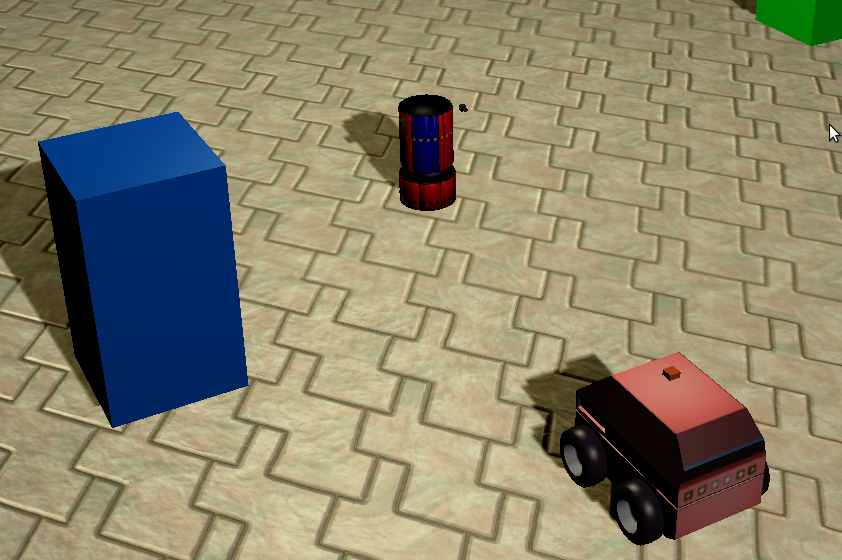
\includegraphics[width=\textwidth]{Bug_Pics/Waypoint/waypoint_1.png}
  \caption{Initial scene.}
\end{subfigure}
~
\begin{subfigure}[!ht]{0.48\textwidth}
  \centering
  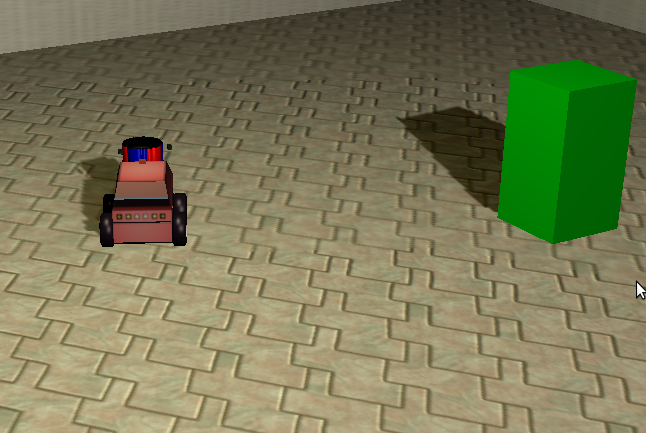
\includegraphics[width=\textwidth]{Bug_Pics/Waypoint/waypoint_2.png}
  \caption{ATRV pushing B21 away.}
\end{subfigure}
\\
\begin{subfigure}[!ht]{1.0\textwidth}
  \centering
  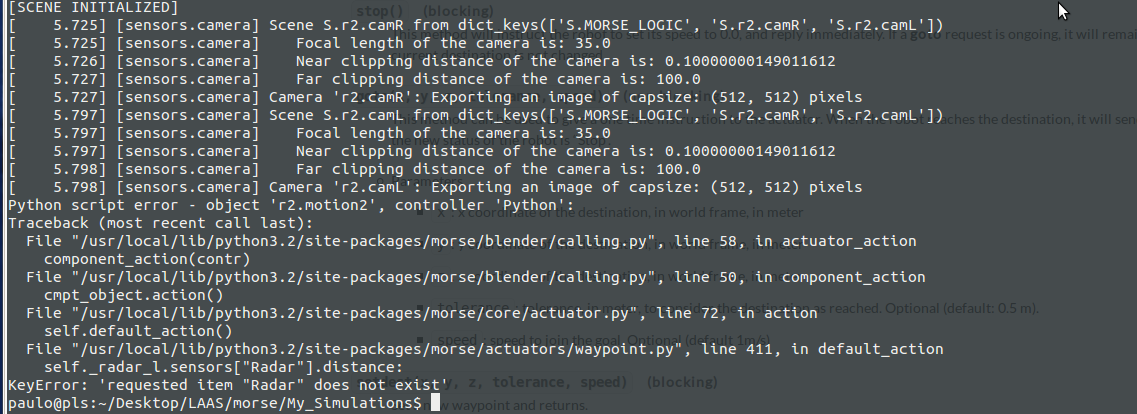
\includegraphics[width=\textwidth]{Bug_Pics/Waypoint/waypoint_3.png}
  \caption{Displayed \textbf{errors} when Blender quits automatically. \label{waypoint_errors}}
\end{subfigure}

\end{center}
\caption{Waypoint failure. \label{Waypoint_failure}}
\end{figure}


\item In \textbf{Supervision \& Communication Services}:
\begin{enumerate}

\item The '\textbf{distance\_and\_view}' service doesn't work so well. See \hyperref[view_bug1]{bug 1} and \hyperref[view_bug2]{bug 2}.

\begin{figure}[!ht] % !-ignore most parameters - here top
\begin{center}
\begin{subfigure}[!ht]{0.48\textwidth}
  \centering
  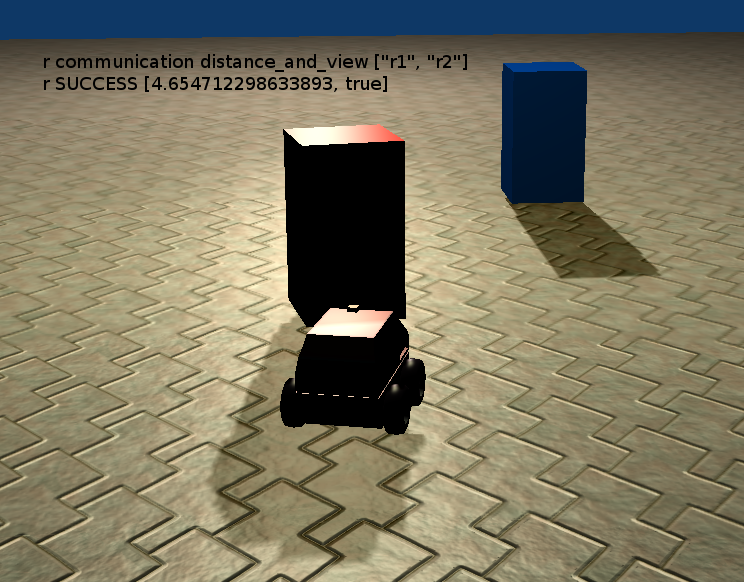
\includegraphics[width=\textwidth]{Bug_Pics/Distance_and_View/distance_and_view_11.png}
  \caption{Picture 1.}
\end{subfigure}
~
\begin{subfigure}[!ht]{0.48\textwidth}
  \centering
  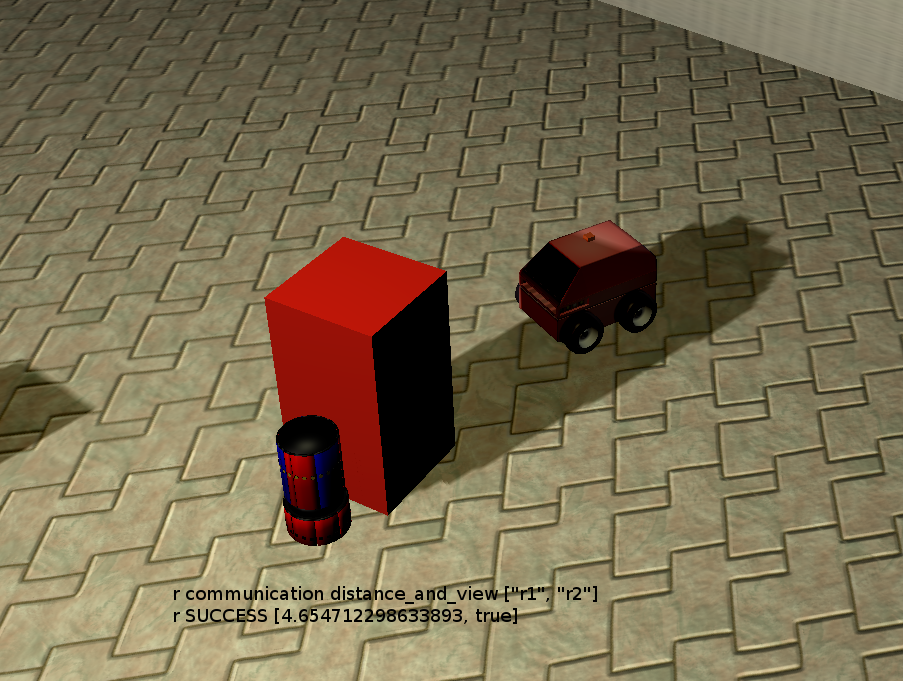
\includegraphics[width=\textwidth]{Bug_Pics/Distance_and_View/distance_and_view_12.png}
  \caption{Picture 2.}
\end{subfigure}

\end{center}
\caption{Bug 1 of \textbf{distance\_and\_view} service. \label{view_bug1}}
\end{figure}

\begin{figure}[!ht] % !-ignore most parameters - here top
\begin{center}
\begin{subfigure}[!ht]{0.48\textwidth}
  \centering
  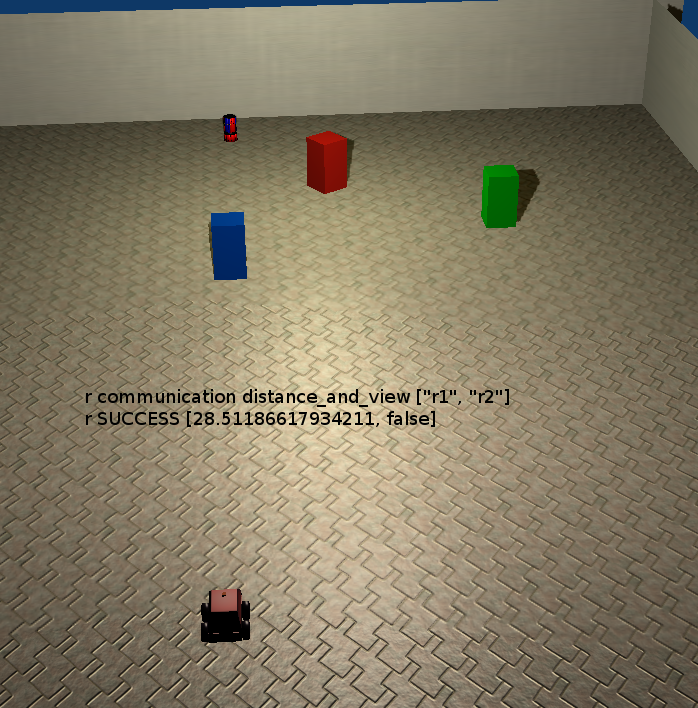
\includegraphics[width=\textwidth]{Bug_Pics/Distance_and_View/distance_and_view_21.png}
  \caption{Picture 1.}
\end{subfigure}
~
\begin{subfigure}[!ht]{0.48\textwidth}
  \centering
  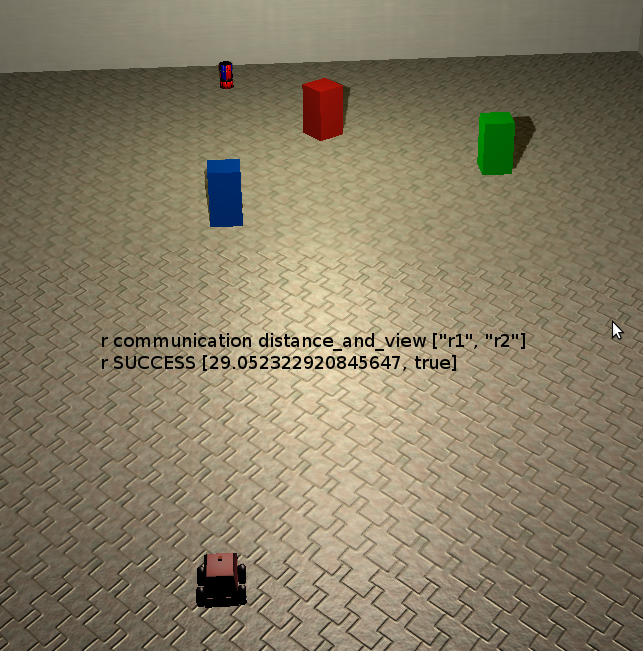
\includegraphics[width=\textwidth]{Bug_Pics/Distance_and_View/distance_and_view_22.png}
  \caption{Picture 2.}
\end{subfigure}

\end{center}
\caption{Bug 2 of \textbf{distance\_and\_view} service. \label{view_bug2}}
\end{figure}

\item When 2 robots can see each other, the service above returns always \textbf{\textit{True}} even if we set a robot as \textit{\textbf{invisible}}. Even if the object will still have physics and dynamics despite being invisible, it is supposed to return true? I also tried with the \textit{\textbf{set\_object\_dynamics}}(off), but it returns true anyway.

\item Using the script above and doing this:
\begin{center}
\$ telnet localhost 4000

r r1.motion1 set\_speed [1, -1]

r SUCCESS

r simulation suspend\_dynamics

r SUCCESS "Physics is suspended"

r simulation set\_object\_dynamics ["r1", 0]

r SUCCESS
\end{center}

I observe all the time that the ATRV robot (r1) never stop doing a circle. Something missing?

\end{enumerate}

\end{enumerate}

